
\chapter{Café Gumbel}

Da unsere Universitätsleitung leider die Meinung vertritt, dass es nicht ihre
Aufgabe ist Studenten  Arbeitsplätze oder Aufenthaltsmöglichkeiten zur Verfügung
zu stellen, ist der einzige Ort, an dem man lernen (reden jedoch nur in
Diskussionsräumen) kann die Bibliothek. Deshalb gibt es in der Theresienstraße
das Café Gumbel (Raum B030).

Das Café Gumbel ist ein vor Jahrzehnten von Studenten erstreikter Raum mit
Küche. Seit einigen Jahren hat die Fachschaft offiziell die Trägerschaft
übernommmen und stellt es euch für diese Zwecke zur Verfügung. Außer
Tischen zum Arbeiten, gemütlichen Sofas zum Entspannen und einem sehr
verstimmten Klavier, ist die Küche populär, die inklusive Wasserkocher und
Geschirr jedem zur Verfügung steht.

Das Gumbel wird auch ab und zu für studentische Veranstaltungen genutzt.
Erwähnenswert sind davon der Spieleabend der Statistiker (nachfragen für
Termine), das weihnachtliche Waffelbacken und das Professorencafé, das einmal
im Jahr stattfindet.  Falls du selbst eine gute Idee für eine weitere
Veranstaltung hast und diese umsetzen möchtest, oder falls du bei einer der anderen
Veranstaltungen mithelfen möchtest, erreichst du die Verantwortlichen über
\mail{gumbel@fs.lmu.de}. Auch beim Betrieb des Gumbel freuen wir uns sehr über
weitere Helfer. Wenn du also oft dort bist, freuen wir uns wenn du uns unter
die Arme greifen willst.

\skiptobottom
\begin{center}
     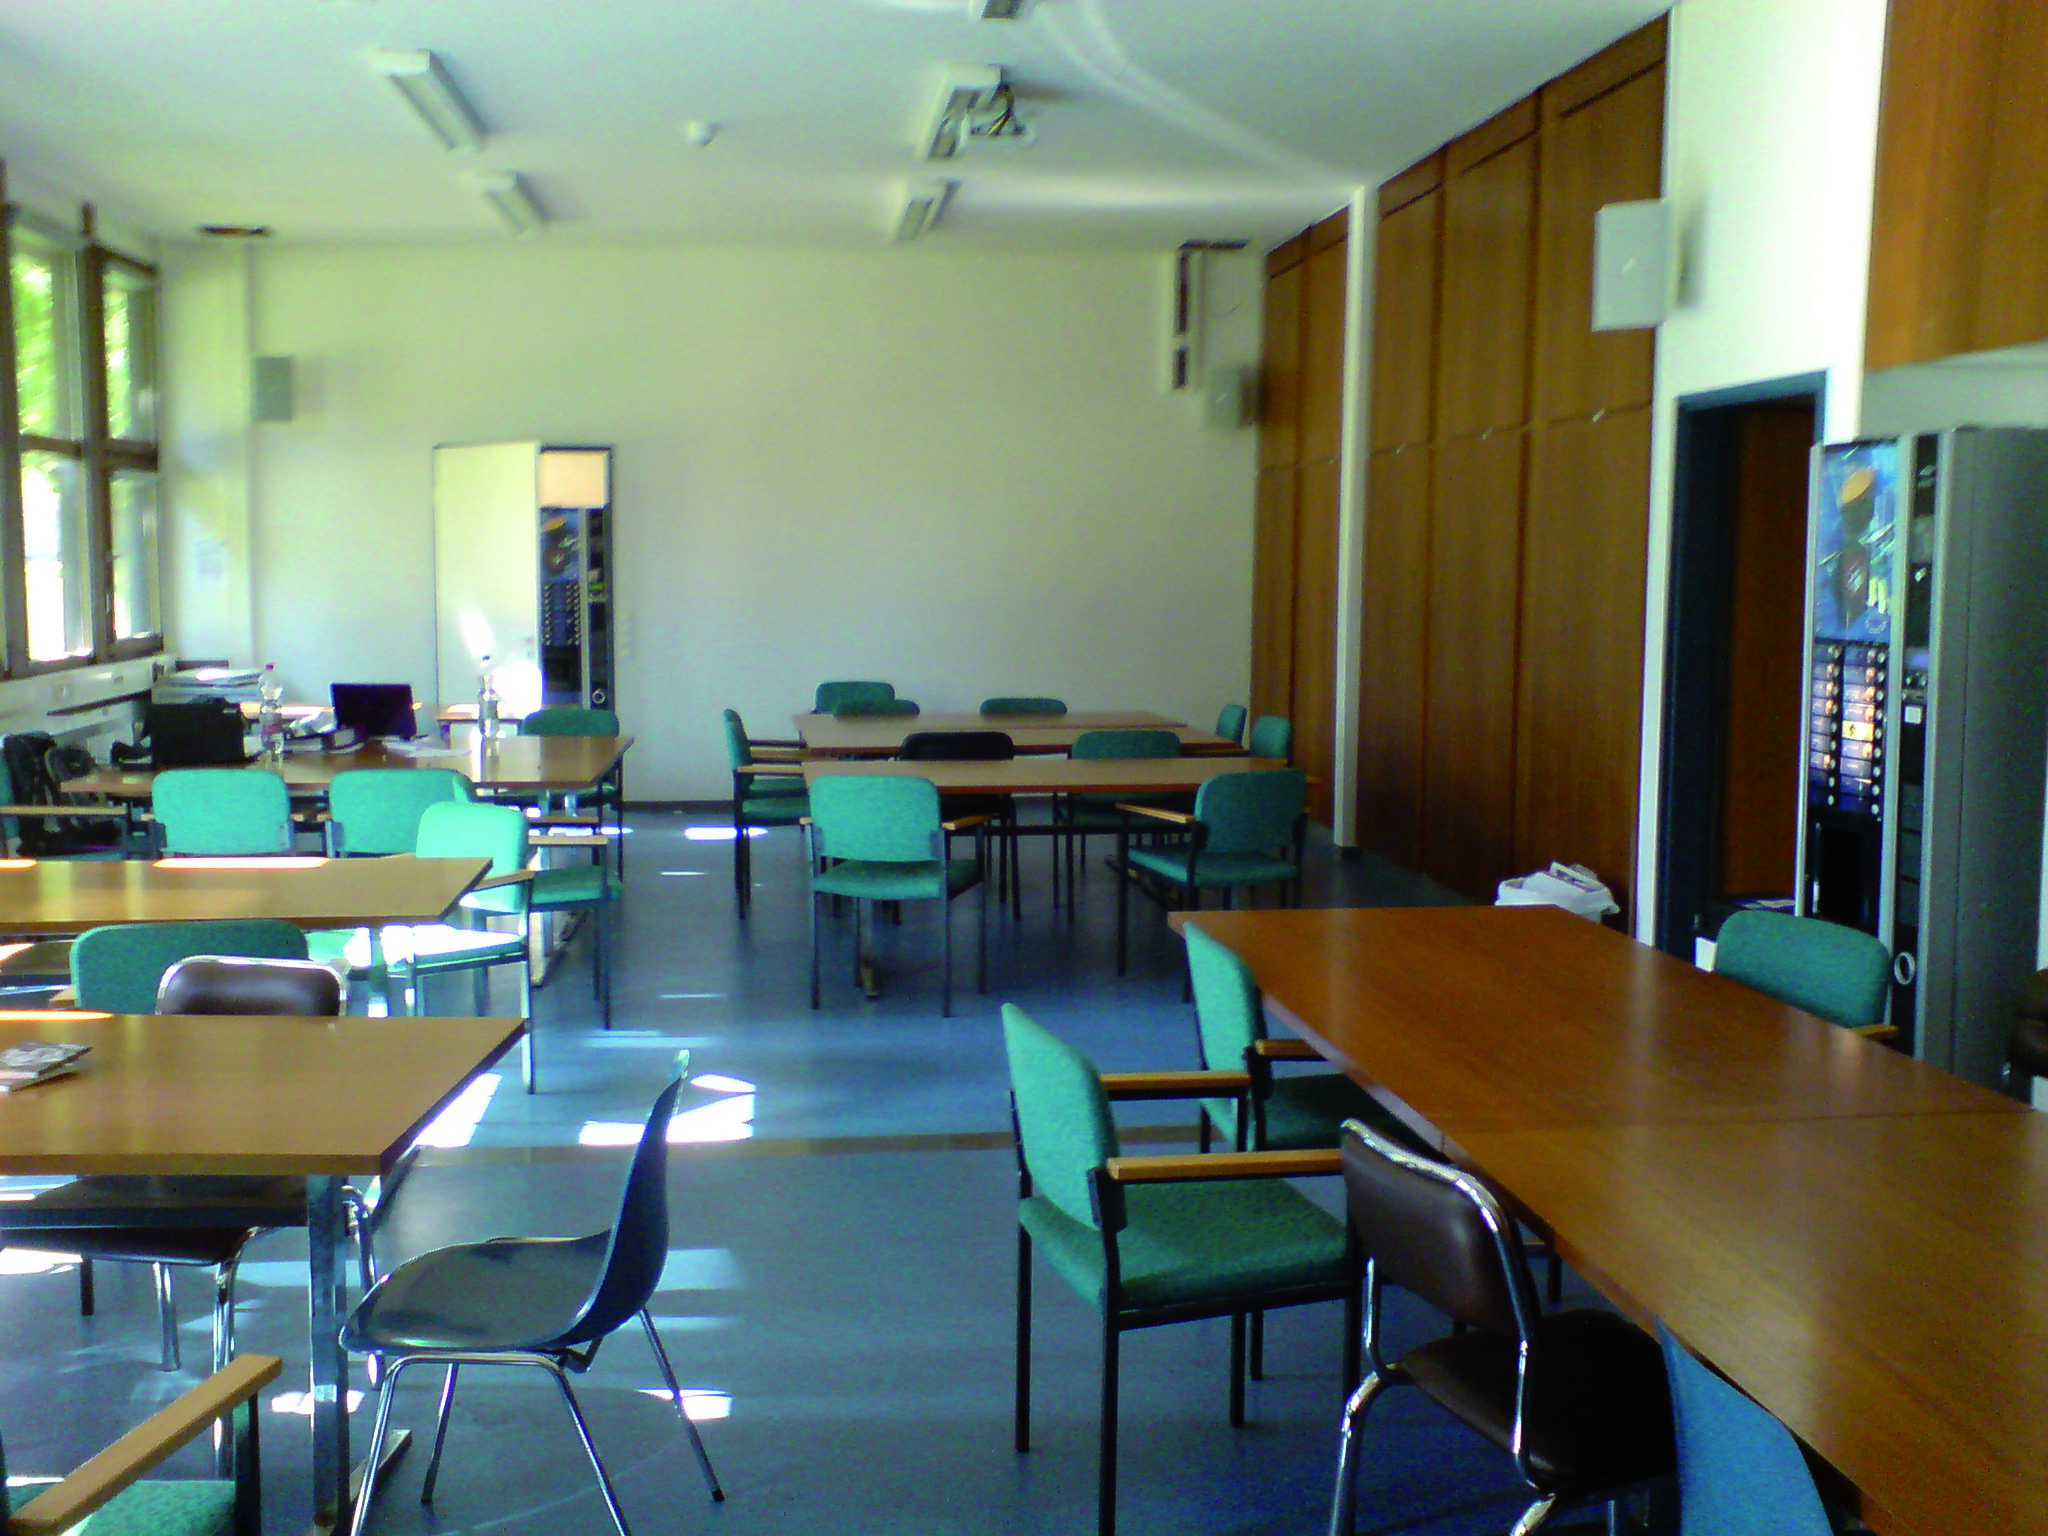
\includegraphics[width=0.96\textwidth]{gumbel_raum_print}
\end{center}